% BottleneckShift technical report. Build: paper/build.sh (Tectonic).
% Every number in the text cites its source report in a comment ("src:").
\documentclass[10pt]{article}
\usepackage[margin=1in]{geometry}
\usepackage[T1]{fontenc}
\usepackage{lmodern}
\usepackage{microtype}
\usepackage{graphicx}
\usepackage{booktabs}
\usepackage{tabularx}
\usepackage{amsmath}
\usepackage[numbers,sort&compress]{natbib}
\usepackage[hidelinks]{hyperref}
\usepackage{xcolor}
\usepackage{enumitem}
\setlist{nosep,leftmargin=*}
\usepackage{caption}
\captionsetup{font=small,skip=4pt}
\setlength{\textfloatsep}{10pt plus 2pt minus 2pt}
\graphicspath{{figures/}}
\newcommand{\ms}{\,ms}

\title{Where Does the Time Go? A Pre-Registered Study of Per-Step Cost in LLM Inference Serving}
\author{Patrick Niyongabo\\Independent researcher, Portland, Oregon\\\url{https://github.com/pniyongabo/BottleneckShift}}
\date{October 2026}

\begin{document}
\maketitle

\begin{abstract}
When an LLM inference server slows down under load, it is often unclear where the time
goes. We measured vLLM serving a 0.5B-parameter model on one GPU in a series of
pre-registered experiments totaling 18{,}900 measured requests. Most runs were
observed from the client, the server's phase metrics, and GPU and CPU telemetry, and
the last experiments added a per-step scheduler log. Every prediction was published
before its data and scored after.

First, from 8 to 32 concurrent requests, past throughput saturation, the added latency
moves into each engine step: the share of latency before the first token falls
from 0.44 to 0.24 while median inter-token latency rises from 4.9 to 55\,ms. Second,
the scheduler's token budget decides where that delay appears. At 32 concurrent
requests, a larger budget gives a 7\,ms median and 18\% more throughput but a
169\,ms 99th percentile, and with the smallest budget queueing takes two thirds of
each request's latency. Third, with one request at a time, a fixed-size prompt chunk
costs up to 1.6$\times$ more at deeper context, in line with a count of attention
FLOPs, and a cost model fit on those data predicts the 99th-percentile inter-token
latency at 8 concurrent requests within 5\% (post hoc). The pre-registered test that a
step's cost tracks its scheduled tokens failed at 8 concurrent requests and passed at
32 with a timing measure we later found lags by one step.

Of 59 scored predictions, 40 held. We report the failures in full, including that
measurement flaw. All GPU time for the study cost \$2.59.
\end{abstract}
% src: counts from the ledger (reports/*); 18,900 = sum of each report's measured requests; numbers from Phase C, Phase D (budget-0512 C32: queue 1222.3 of mean E2E 1843.9 ms), and Milestone 5 reports

\section{Introduction}
\label{sec:intro}

LLM serving systems batch many requests through one model. Each engine step generates
one token for every running request and may also process part of a new request's
prompt \citep{yu2022orca,kwon2023vllm,agrawal2024sarathiserve}. Service targets are
usually written in terms of time to first token (TTFT) and time per output token
\citep{zhong2024distserve}. A user feels both the wait for the first token and how
smoothly the rest stream. An operator who sees latency rise therefore needs to know
which phase grew and why. Past saturation the excess work is the same either way. The
scheduler decides whether it appears as waiting before the first token or as slower
steps, and its settings move it between the two.

This report asks under which conditions the dominant source of client-visible delay
changes, and which measurements can tell the causes apart. We
answer it for one setup, vLLM serving Qwen2.5-0.5B-Instruct on one RTX A4000. We use a
method designed to make negative results visible. Each experiment's predictions and
thresholds were published before its data were collected, runs were measured from
three independent views, and every prediction was scored afterward, including the
ones that failed.

Our contributions are:
\begin{itemize}
  \item \emph{A pre-registered, three-view measurement method} for LLM serving, with
    an opt-in per-step scheduler log that records how many tokens each engine step
    processed and when its results returned (Section~\ref{sec:method}).
  \item \emph{Where latency goes under load:} from C8 to C32, past saturation, the
    added latency appears as per-step time while the share before the first token
    falls, and a capacity argument bounds how far this extends
    (Section~\ref{sec:load}).
  \item \emph{The token budget as a median-versus-tail trade:} at C32 the budget sets
    the scale of the inter-token latency tail, and the smallest budget moves the delay
    into the queue (Section~\ref{sec:budget}).
  \item \emph{What sets the cost of a step:} context, measured directly for single
    chunks and consistent with a FLOP count, and what the step log could and could
    not show about scheduled tokens (Section~\ref{sec:stepcost}).
  \item \emph{A prediction ledger:} all 59 scored predictions and what the 19 that did
    not fully hold taught us (Section~\ref{sec:ledger}).
\end{itemize}
The code, configurations, protocols, and reports are public.\footnote{\url{https://github.com/pniyongabo/BottleneckShift}}
% src: ledger counts (40 confirmed, 4 mixed, 14 not confirmed, 1 not testable)

\section{Background}
\label{sec:background}

\paragraph{Phases and steps.}
vLLM runs in \emph{engine steps}: each step, the scheduler picks the tokens to process
and the model runs one forward pass over all of them. A request first waits in a
\emph{queue}. Its \emph{prefill} phase processes the prompt and produces the first
output token. Its \emph{decode} phase then produces each remaining output token in one
step, so a request with 32 output tokens spends 31 steps in decode. With chunked
prefill \citep{agrawal2024sarathiserve}, a long prompt is split across several steps,
and one step can carry both decode tokens and prompt chunks.

\paragraph{Token budget.}
The \emph{token budget} $B$ (vLLM's \texttt{max\_num\_batched\_tokens}) is the most
tokens one step may process: one per decoding request plus every prompt token in the
step's chunks. Its default in our configuration is 2048. The scheduler fills each step
first with running requests (one token per decoding request, or the next chunk of a
prompt in progress) and then with waiting prompts, until the budget is used. A step
that carries a large chunk takes about as long as a prefill, and every request decoding
in that step waits for it. vLLM's documentation says smaller budgets give better
inter-token latency and larger ones better TTFT and throughput
\citep{vllmdocsoptimization}.

\paragraph{Metrics.}
Client metrics come from vLLM's benchmark. TTFT runs from sending a request to
receiving its first token, and E2E to receiving its last. Inter-token latency (ITL) is
each gap between consecutive tokens of a request; time per output token (TPOT) is a
request's average gap, $(\mathrm{E2E}-\mathrm{TTFT})/(n-1)$ for $n$ output tokens. We
report ITL percentiles, the median (p50) and 99th percentile (p99), because averages
hide jitter \citep{agrawal2024etalon}. The benchmark pools the gaps of all requests in a
run, and one step produces a gap for every request decoding in it, so a run's ITL p99
reflects its slowest few steps; where we give a mean ITL, it nearly equals the mean
TPOT. The \emph{share of latency before the first token} is $\sum \mathrm{TTFT} / \sum
\mathrm{E2E}$ over a run's requests. On the server, vLLM's histograms split each
request into queue, prefill (from first being scheduled to the first token), and
decode (from the first token to the last) time.

\section{Method}
\label{sec:method}

\paragraph{Setup.}
All experiments used a rented NVIDIA RTX A4000 (16\,GB) with the NVIDIA 580-series
driver and vLLM 0.29.0, serving Qwen2.5-0.5B-Instruct. Sessions ran on several rented
virtual machines, each with its own physical GPU; Phase C reused Phase B's machine. The
client was \texttt{vllm bench serve} on the same host, issuing a closed-loop workload.
Up to a fixed number of requests (the concurrency, written C1 to C32) are kept in
flight, and a new request is sent as soon as one finishes. Each run sends 100 requests
(50 for the decode-heavy workload), so a run at C32 starts with a burst of 32 requests
and ends as the last ones drain. Prompts are synthetic, with exact input and output
lengths and a fixed seed.
% src: configs/*.toml (num_prompts 100; 50 for decode-heavy); reports/milestone1-*.md (driver 580.178.04); reports/milestone2-*.md (different physical GPU); reports/milestone3-*-phase-c.md (same VM as Phase B); reports/milestone5p2-*-part2.md (Provenance)

\paragraph{Controls.}
A first baseline (Milestone 1) compared C1 with C8, in forward and reverse order with
three repetitions and 15-second cooldowns, and found 6.65$\times$ higher output
throughput at C8. It ran with prefix caching on, an unpinned model revision, and the
model's own sampling defaults (temperature 0.7, top-p 0.8, top-k 20, repetition
penalty 1.1), any of which could inflate or mask the effect. A controlled repeat
(Milestone 2) turned prefix caching off, pinned the server's model and tokenizer revisions,
used greedy sampling, ignored the model's generation defaults
(\texttt{--generation-config vllm}), and warmed up at each measured concurrency. The
effect held (about 6.5$\times$), and these controls are fixed in every later run.
% src: reports/milestone1-20261001T205137Z.md (Result: 6.65x); reports/milestone2-20261003T034456Z.md (~6.5x); experiments/roadmap.md

\paragraph{Pre-registration.}
Each phase's protocol was merged into the public repository before its data were
collected. Milestones 1 and 2 stated expected signatures; from Milestone 3 on, each
protocol has predictions with thresholds and falsification rules (Phase B states them
as signatures for each workload regime). The merge
time is the evidence of pre-registration. Each Milestone 3 and 5 report scores every prediction as
confirmed, mixed, or not confirmed (with a few qualified verdicts, such as "not
testable"), and marks interpretations made after seeing the data as post hoc.
Section~\ref{sec:ledger} collects the 59 scored predictions of Milestones 3 and 5.

\paragraph{Three views of every run.}
From Milestone 3 on, each run is measured three ways.
\begin{itemize}
  \item \emph{Client:} time to first token (TTFT), the gaps between streamed tokens
    (inter-token latency, ITL; we report the median, p50, and the 99th percentile,
    p99), end-to-end latency (E2E), and output throughput.
  \item \emph{Server:} vLLM's Prometheus histograms for queue, prefill, and decode
    time per request, scraped before and after each run.
  \item \emph{Resources:} GPU utilization from \texttt{nvidia-smi} every 200\,ms,
    and CPU utilization every second.
\end{itemize}

\paragraph{A per-step scheduler log.}
vLLM's per-iteration token histogram credits a request's whole prompt to the step that
emits its first token, so it cannot show how many prompt tokens a step actually
processed. A manipulation check that relied on it failed as specified
(Section~\ref{sec:budget}). For Milestone 5 we added an opt-in vLLM plugin that wraps
the scheduler and writes one line per engine step, recording the scheduled tokens
(split into prefill and decode) and the scheduled requests. Part~2 added each prefill
chunk's context position and the time the step's results returned.
From these we compute a step's \emph{execution time}: the time from when it could
start (it was scheduled and the previous step's results had arrived) until its own
results arrived. Unlike the interval between scheduling calls, this measure is tied to
the step itself even when vLLM schedules the next step early. vLLM 0.29.0 can schedule
a step before the previous step's results return; we did not record which scheduling
mode was active.
% src: reports/milestone3-*-phase-d.md (iteration histogram); experiments/milestone5.md (Instrument; Part 2 addendum)

\paragraph{Validation and provenance.}
Every series is validated before analysis. The validator checks:
\begin{itemize}
  \item that runs completed with zero failures and exact token lengths;
  \item that the server's request count matches the prompts sent;
  \item that warm-ups ran and telemetry covers the series (sampling gaps of up to
    1\,s for the GPU and 3\,s for the CPU are allowed);
  \item for Milestone 5, that the step log covers every measured run.
\end{itemize}
Raw results are archived with a SHA-256 checksum, verified after transfer, before the
machine is deleted. Across all sessions the study comprises 18{,}900 measured requests.
% src: measured-request counts from each report's Validation table: M1 1,200; M2 1,200; B 1,800; C 4,800; D 5,400; M5 pilot 2,100; M5 Part 2 2,400

\section{Where latency goes under load}
\label{sec:load}

\paragraph{Decode dominates each request, even with long prompts.}
We first compared a prefill-heavy workload (2048 input and 32 output tokens) with a
decode-heavy one (64 and 512), at C1 and C8. We had predicted that the prefill-heavy
workload would be dominated by the time before the first token. It was not. A request
running alone spent about 40\ms{} in prefill and about 122\ms{} in its 31 generation
steps. A simple cost estimate predicts this \citep{pope2023scaling}. Prefill of 2048
tokens needs about 1.6 TFLOP (two FLOPs per weight per token, plus attention), which
takes 21\ms{} at the A4000's dense 16-bit tensor peak of 77 TFLOPS. Each generation step
must read about 1\,GB of weights, which takes at least 2.2\ms{} at 448\,GB/s, or
68\ms{} for 31 steps \citep{nvidiaa4000}. At those ideal rates prefill would be about
a quarter of the request, so on this GPU the workload we called prefill-heavy is
decode-dominated, and the prediction could have been made from the estimate.

At C8 the share of latency before the first token rose from 31\% to 45\%, but it
stayed below half. (At C1 the client's TTFT of 54\ms{} includes about 14\ms{} of request
handling outside the server's prefill time.) Concurrency did amplify different
components in the two regimes. The decode-heavy workload gained 6.46$\times$
throughput from C1 to C8 for 10\% slower per-token time. The prefill-heavy one gained
only 2.8$\times$, with queueing and a tenfold rise in ITL p99.
% src: reports/milestone3-20261003T180358Z-phase-b.md (Result; predicted signatures table; C1 TTFT 54.4 ms, server 0.01 / 40.3 / 122.5 ms); FLOP and byte estimate from the model config (24 layers, hidden 896, MLP 4864, 0.36B non-embedding and 0.49B total parameters, bf16) and the A4000 datasheet (448 GB/s; 153.4 TFLOPS tensor with sparsity, so 76.7 dense)

A plausible reading at the time is that at C8 much of a request's decode time is spent
in engine steps that also carry other requests' prompt chunks. Under chunked prefill,
vLLM schedules running decodes and new prompt chunks in the same step, up to its token
budget. A step that carries a large chunk takes about as long as a prefill, so every
request decoding in that step sees a long inter-token gap. A per-request phase
breakdown therefore books much of the GPU's prefill work as decode time. Milestone 5's
step log fits this reading: at this prompt length, 23\% of C8 steps carried prompt
work.
% src: reports/milestone3-*-phase-b.md (Interpretation: what server decode time measures at C8); reports/milestone5p2-*-part2.md (C8 step-log table, len2048-budget2048-c8: 23%)

\paragraph{Past saturation, the added latency moves into each step.}
We then raised concurrency on the prefill-heavy workload to C16 and C32, predicting
that the time before the first token would come to dominate. The opposite happened.
The share of latency before the first token fell from 0.44 at C8 to 0.35 at C16 and
0.24 at C32. Output throughput peaked at C16 (583 tokens/s) and fell slightly at C32
(555). Median ITL went from 4.9\ms{} at C8 and 5.5\ms{} at C16 to 55\ms{} at C32
(Figure~\ref{fig:crossover}). A pre-registered sweep (C8, C12, C16, C24, C32) located
the jump between C16 (5.5\ms) and C24 (45.8\ms). It reproduced the earlier session
within about 1\% on a different machine. The jump in the median is abrupt because the
gaps form two clusters, short ones from decode-only steps and long ones from steps that
carry a prompt chunk, and the median moves from one cluster to the other once most
gaps come from prompt-carrying steps. Server decode time per output token rose more
smoothly, from 8.7\ms{} at C8 to 18.1\ms{} at C16 and 44.7\ms{} at C32.
% src: reports/milestone3-20261003T201214Z-phase-c.md (Result; crossover table; server decode 270.9 / 559.7 / 1384.8 ms over 31 steps); reports/milestone3-20261006T022744Z-phase-d.md (sweep; prediction 1; reproduction)

\begin{figure}[t]
  \centering
  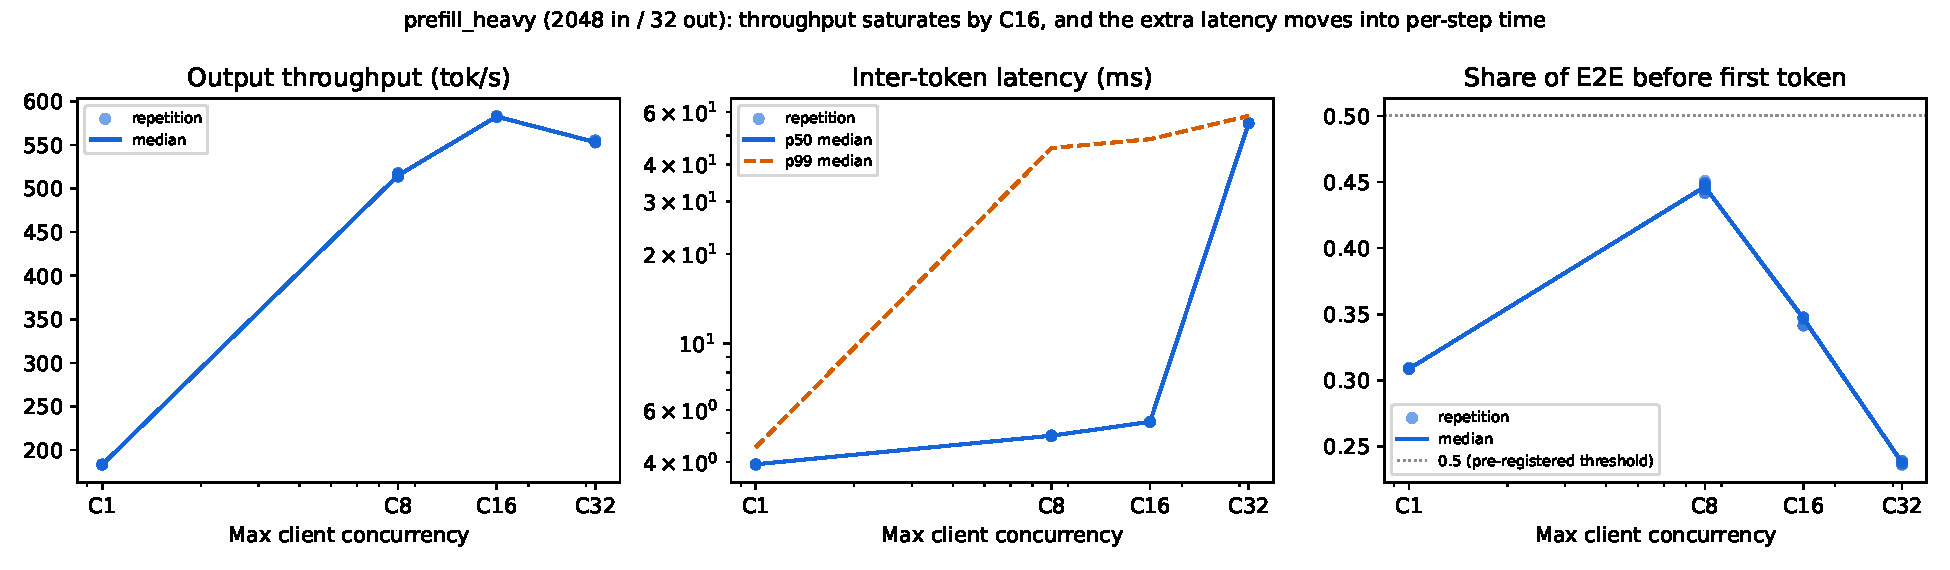
\includegraphics[width=0.78\linewidth]{milestone3-phase-c-crossover.pdf}
  \caption{Prefill-heavy workload (2048/32 tokens) against concurrency: output
    throughput, ITL p50 and p99, and the share of latency before the first token.
    Past C16, added latency appears as per-step time while the share before the
    first token falls. The C1 points and six of the twelve C8 points come from the
    contention study's control series.}
  \label{fig:crossover}
\end{figure}

\paragraph{The shift is bounded.}
At $B{=}2048$ a step carries at most one 2048-token chunk, so it costs at most about
56\ms{} (ITL p99 was 58\ms{} at C32), and a request's 31 generation steps take at most
about 1.8\,s. Past saturation throughput no longer grows, so by Little's law each added
request in flight adds latency, and once steps are full that latency must go into the
wait for the first token. Mean TTFT already doubled from C8 (215\ms) to C32
(431\ms). The per-step shift we measured therefore describes C16 to C32 at this budget,
while steps fill toward the cap. Beyond C32, and under open-loop load, we expect delay
to return to TTFT; we did not test this.
% src: reports/milestone3-20261003T201214Z-phase-c.md (crossover table: mean TTFT 215.2 / 430.9 ms; ITL p99 58.2 ms at C32); bound derived from the budget cap

\section{The token budget reshapes per-step cost}
\label{sec:budget}

vLLM caps the tokens one engine step may process with \texttt{max\_num\_batched\_tokens},
the token budget $B$. Its default on this GPU is 2048, which equalled the prompt
length in the experiments above. If the jump in per-step time comes from steps that
carry prompt chunks, the budget should control it.

\paragraph{Median against tail.}
At C32 we set the budget to 512, 2048, and 8192 (Table~\ref{tab:budget}). No setting wins on every metric:
\begin{itemize}
  \item \emph{512:} spreads prompt work into many small steps. ITL is nearly flat
    (p50 15.8\ms, p99 17.8\ms), but TTFT triples and throughput falls 10\%. Queueing
    takes two thirds of each request's latency (1.2 of 1.8\,s).
  \item \emph{2048 (the default):} most steps carry a full 2048-token chunk, so p50
    and p99 are both near 55--59\ms.
  \item \emph{8192:} batches several prompts into fewer, much larger steps. The
    median falls to 6.9\ms{} and throughput rises 18\%, but p99 rises to 169\ms.
\end{itemize}
The budget with the best median has the worst tail. By mean time per output token
after the first, $(\mathrm{E2E}-\mathrm{TTFT})/31$, the order is 512 (15\ms), 8192
(26\ms), and 2048 (45\ms). These descriptions of how each budget cuts prompt work into
steps were Phase D's post hoc reading; Milestone 5's step log later showed the step
sizes directly: at 2048, 77\% of steps carried prompt work, with a median of 2048
prompt-carrying tokens (Section~\ref{sec:stepcost}).
% src: reports/milestone3-20261006T022744Z-phase-d.md (Result table: queue 1222.3 of E2E 1843.9 ms at 512; mean E2E and TTFT per budget; prediction 7; prediction 10); reports/milestone5-*-pilot.md (step-log table, anchor-before)

\begin{table}[t]
  \centering
  \caption{Token budget at C32, prefill-heavy workload (2048/32 tokens). Medians of
    three repetitions.}
  \label{tab:budget}
  \begin{tabular}{rrrrr}
    \toprule
    Budget & ITL p50 (ms) & ITL p99 (ms) & Mean TTFT (ms) & Output tok/s \\
    \midrule
    512  & 15.8 & 17.8  & 1378.8 & 496.2 \\
    2048 & 55.4 & 58.6  & 432.7  & 550.8 \\
    8192 & 6.9  & 168.7 & 686.1  & 652.5 \\
    \bottomrule
  \end{tabular}
  % src: reports/milestone3-20261006T022744Z-phase-d.md (Part 2 table; predictions 7, 8, 10; Phase C bullet: 652.5 tok/s at 8192)
\end{table}


We had predicted that both ITL p50 and p99 would order 512 $<$ 2048 $<$ 8192. The
p99 ordering held and the p50 ordering did not. The manipulation check relied on
vLLM's iteration-token histogram, which cannot show per-step chunk sizes
(Section~\ref{sec:method}), and it failed as specified. Under the pre-registered rule,
that made the test of the mechanism inconclusive. If we accept server-log evidence
that the budgets were applied, which is a deviation from the protocol, the
pre-registered form of the step-size explanation, a p50 that rises with the budget, is
unsupported. The measured trade-off stands, and the open mechanism
motivated Milestone 5.
% src: reports/milestone3-*-phase-d.md (Falsification; prediction 6 failed as specified; prediction 7)

\paragraph{Prompt length against budget.}
Milestone 5 varied the prompt length $L \in \{1024, 2048, 4096\}$ at budgets 2048 and
8192 with the step log enabled (Table~\ref{tab:lengths}, Figure~\ref{fig:pilot}).
\begin{itemize}
  \item \emph{The budget sets the scale of the tail.} At $B{=}2048$, ITL p99 was
    58\ms{} for 2048-token prompts and 65\ms{} for 4096-token prompts. Past the budget,
    prompts are split into budget-sized chunks, so the tail grew only 11\%. At
    $B{=}8192$ the tail was about 3$\times$ higher (170 and 200\ms), while the median
    stayed below 10\ms.
  \item \emph{Prompts shorter than the budget did not shrink the tail as predicted.}
    The pre-registered prediction was that 1024-token prompts would have a tail at
    least 25\% lower than 2048-token prompts. It was 19\% lower. The step log suggests why
    (a post hoc reading): the scheduler packed two 1024-token prompts into one
    2048-token step (Section~\ref{sec:stepcost}).
  \item \emph{Concurrency moves the median.} At C8 with $B{=}2048$, ITL p50 was
    4.6--5.7\ms{} for every prompt length, against 55--57\ms{} at C32 for $L \ge 2048$
    (6.1\ms{} at $L{=}1024$, where prompts are packed), as predicted; only a minority
    of C8 steps carry prompt work. The tail fell less, to 40--54\ms. 1024-token prompts
    were packed at C8 as well (an 11\% lower tail, against a predicted 25\%). At C8
    with $B{=}8192$, prompt length did move the tail: p99 rose from 60 to 178\ms{}
    between $L{=}1024$ and $L{=}4096$.
\end{itemize}
% src: reports/milestone5-20261025T004640Z-pilot.md (Measurements; predictions 3-5); reports/milestone5p2-20261029T000043Z-part2.md (C8 table; predictions 8, 9)

\begin{table}[t]
  \centering
  \caption{Prompt length $L$ against budget $B$ at C32 and C8 (32 output tokens).
    ITL p50 / p99 in ms; medians of three repetitions.}
  \label{tab:lengths}
  \begin{tabular}{rrrr}
    \toprule
    $B$ & $L$ & C32 & C8 \\
    \midrule
    2048 & 1024 & 6.1 / 47.4  & 4.6 / 40.4 \\
    2048 & 2048 & 55.3 / 58.3 & 4.9 / 45.5 \\
    2048 & 4096 & 57.4 / 64.7 & 5.7 / 53.8 \\
    8192 & 1024 & 5.7 / 151.3 & 4.6 / 60.4 \\
    8192 & 2048 & 7.0 / 169.5 & 4.9 / 120.3 \\
    8192 & 4096 & 9.7 / 199.9 & 5.5 / 177.5 \\
    \bottomrule
  \end{tabular}
  % src: reports/milestone5-20261025T004640Z-pilot.md (Measurements, C32; L2048/B2048 is anchor-before); reports/milestone5p2-20261029T000043Z-part2.md (Part 2A table, C8)
\end{table}

\begin{figure}[t]
  \centering
  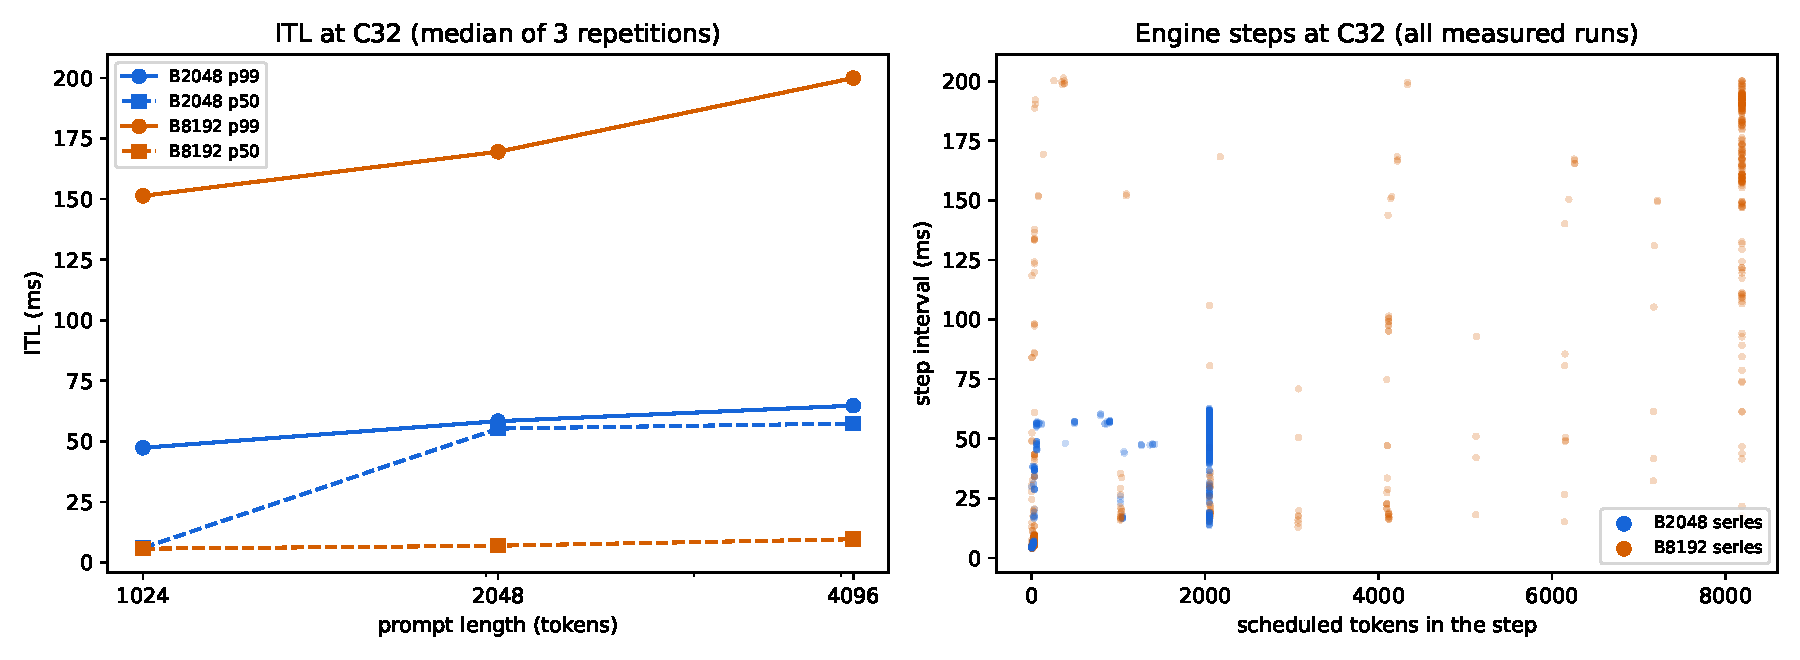
\includegraphics[width=\linewidth]{milestone5-pilot.pdf}
  \caption{Milestone 5 at C32. Left: ITL p50 and p99 by prompt length for each
    budget. Right: every measured engine step's interval (to the next step's start)
    against its scheduled tokens. This interval is confounded with the previous step
    (Section~\ref{sec:stepcost}).}
  \label{fig:pilot}
\end{figure}

\section{What sets the cost of a step}
\label{sec:stepcost}

\paragraph{Step size.}
The step log confirmed the budget was applied exactly. No step scheduled more than $B$
tokens, and each run's logged prompt tokens equalled the number sent. The primary
prediction of Milestone 5 was that a step's cost tracks its scheduled tokens, measured
by the interval from one scheduling call to the next. Pooled over the seven C32
series, steps of at least 1024 tokens were followed by a median interval of 56\ms,
against 5.7\ms{} for steps of at most 64 tokens (9.8$\times$, Spearman 0.87), and the
prediction passed. At C8 the same test gave 9.0$\times$ but a Spearman correlation of
0.57, below its threshold of 0.7. Under the protocol's rule, this rejects the
hypothesis's first clause at C8.
% src: reports/milestone5-20261025T004640Z-pilot.md (predictions 1, 2); reports/milestone5p2-*-part2.md (prediction 2; Result: the pre-registered rule rejects H's first clause at C8); experiments/milestone5.md (falsification rule)

\paragraph{A lagged measure.}
The interval is confounded with the previous step. vLLM 0.29.0 can schedule step
$n{+}1$ before it processes step $n$'s results, so the interval credited to step $n$
partly reflects the cost of step $n{-}1$. The pilot found that the interval correlated
better with the previous step's tokens (0.92) than with the step's own (0.87). Some
intervals are too short to be a step's own cost: at C8 with $B{=}8192$ and $L{=}1024$,
steps of at least 1024 tokens had a median interval of 16.5\ms, while a single
1024-token chunk took a median of at least 19.5\ms{} at every context we measured
(below). At C32, prompt-carrying steps come in runs, so a lagged measure still
separates large steps from small ones, and the C32 pass is weak evidence about a
step's own cost. Part~2's execution time is tied to the step itself
(Section~\ref{sec:method}). Over the C8 block it tracked a step's own tokens better
than the interval did (Spearman 0.63 against 0.57), still below the threshold. No C32
run recorded it.
% src: reports/milestone5-*-pilot.md (Interpretation: measurement note); reports/milestone5p2-*-part2.md (C8 step-log table: len1024-budget8192-c8 16.5 ms; Part 2B table; prediction 14); vLLM 0.29.0 v1/engine/core.py (step_with_batch_queue)

\paragraph{Packing (post hoc).}
The step log also suggests why part of the tail prediction failed. At $B{=}2048$ and
$L{=}1024$, 94\% of steps carrying at least 1024 prompt tokens held two or more
prompts, and the median prompt-carrying step was a full 2048 tokens. vLLM's scheduler
fills the budget whenever prompts are waiting, so a prompt shorter than the budget
changes how often steps carry prompt work (38\% of steps at $L{=}1024$, against 77\%
at $L{=}2048$) more than how large those steps are. This fits the median falling far
(6.1 against 55\ms) while the tail fell only 19\%. Our workload favors packing: all
requests have the same lengths and start together, so they finish and return in
groups. With staggered arrivals, fewer prompts would wait at once.
% src: reports/milestone5-20261025T004640Z-pilot.md (Interpretation: short prompts are packed; step-log table)

\paragraph{Context.}
The pilot had suggested a role for context: 2048-token steps were followed by shorter
intervals at shorter prompts (45\ms{} at $L{=}1024$, 55.5\ms{} at $L{=}2048$). We
withdraw that reading. At both lengths those steps start at context 0, and the gap
follows the share of steps that carry prompt work (38\% against 77\%), as a lagged
measure would. A second pre-registered design tested context directly. We ran one
request at a time (C1) with 8192-token prompts at budgets 1024 and 2048, so every
prompt step held exactly one chunk of exactly $B$ tokens at a known context position,
and timed each chunk by its execution time (Figure~\ref{fig:context}). Chunk cost rose
almost linearly with context:
\begin{itemize}
  \item 1024-token chunks took 25.0\ms{} at context 0 and 19.5\ms{} at context
    1024, then rose to 35.9\ms{} at context 7168;
  \item 2048-token chunks rose from 41.7\ms{} at context 0 to 67.4\ms{} at context
    6144.
\end{itemize}
The deepest chunk cost 1.44$\times$ and 1.62$\times$ the first, and the Spearman
correlation between context and execution time was 0.96 in both series. From context
2048 on, each additional 1024 tokens of context added about 1.9\ms{} to a 1024-token
chunk and 3.8\ms{} to a 2048-token chunk.
% src: reports/milestone5-*-pilot.md (step-log table: 44.9 / 55.5 ms; 38% / 77%); reports/milestone5p2-20261029T000043Z-part2.md (Part 2B table; predictions 11-13; Interpretation: slopes)

These slopes match a FLOP count. A chunk of $n$ tokens at context $c$ spends about
$4ncd$ attention FLOPs per layer on the prior context, with $d{=}896$ and 24 layers.
Each 1024 tokens of context then costs 0.09 TFLOP for a 1024-token chunk and 0.18
TFLOP for a 2048-token chunk. At the tensor peak these take 1.2 and 2.4\ms; at the
40 TFLOPS that the context-0 2048-token chunk achieved, 2.3 and 4.6\ms. The measured
slopes lie between the two and double with chunk size, as the count predicts. The
first chunk of each prompt was slower than the second at $B{=}1024$ (25.0 against
19.5\ms), plausibly because of per-request setup on a request's first step; this
reading is post hoc. That setup cost lowers the ratios measured from context 0: taken
from the second chunk, the $B{=}1024$ ratio is 1.84$\times$, and at context 0 a
2048-token chunk cost 1.67$\times$ a 1024-token chunk, where FLOPs predict about
2.1$\times$.
% src: FLOP count from the model config (14 heads of 64 dimensions, 24 layers) and the A4000 datasheet; 40 TFLOPS = (1.47 linear + 0.18 attention TFLOP) / 41.7 ms; 1.84 = 35.9 / 19.5

\begin{figure}[t]
  \centering
  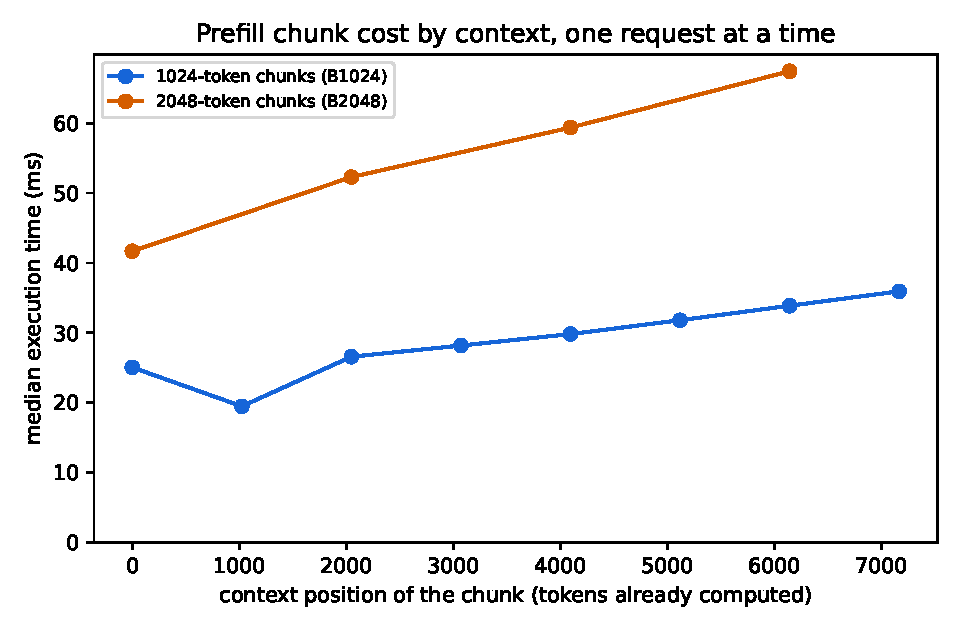
\includegraphics[width=0.55\linewidth]{milestone5-part2-context.pdf}
  \caption{Median execution time of prefill chunks by context position, one request
    at a time with 8192-token prompts (300 chunks per point).}
  \label{fig:context}
\end{figure}

\section{A secondary finding: GPU contention}
\label{sec:contention}

We also ran a co-located synthetic GPU job alongside the prefill-heavy workload, with a
sham condition and a recovery baseline. The job was busy for 25\% or 50\% of each
100\,ms period, and its kernels ran 14\% and 28\% of the time. The two processes share
the GPU by time-slicing \citep{nvidiatimeslicing}. At the 50\% setting:
\begin{itemize}
  \item the job cost 13--15\% in end-to-end latency;
  \item it slowed requests even at C1, and at C1 it slowed prefill more than decode
    (+22.5\% against +11.3\%); we have no tested explanation for the difference;
  \item mean \texttt{nvidia-smi} utilization moved by only 1--6 points, against a
    3.5-point spread between identical control runs. Without contention it was
    already about 90\% at C1 and higher at C8, which leaves little room to move.
\end{itemize}
Of seven predictions, four held, two were mixed, and one failed. Utilization stayed
within 5 points at C1 but moved 6.0 points at C8. Queue time at C8 rose only 6\%,
less than prefill (+17\%), against the prediction. The share of latency before the
first token did not rise, which was the one outright failure. We state this contrast
with added load for our closed-loop client; an open-loop test would check it. Near its
ceiling, utilization is a poor detector of this interference \citep{nvidiasmi}.
% src: reports/milestone3-20261003T201214Z-phase-c.md (Result; validation table: kernel duty 0.142 at 0.25; Part 2 table: control utilization 88.3-91.8% at C1; Part 2 predictions 3, 5; Interpretation: contention signature, closed loop, utilization)

\section{The prediction ledger}
\label{sec:ledger}

Table~\ref{tab:ledger} counts every scored prediction by phase. Of 59 verdicts, 40
were confirmed, 4 were mixed, 14 were not confirmed, and 1 could not be tested with
our instruments. We group the misses below by what caused them; the reports discuss
each one, including those that fit no group, such as the order of TTFT across
budgets.

\begin{table}[t]
  \centering
  \caption{Scored predictions by phase. Phase B scores ten signatures for each of two
    workload regimes. Milestone 5's C8 predictions are counted in Part~2. Where a
    report gives a split or qualified verdict (Phase D predictions 2 and 7), we count
    it as mixed.}
  \label{tab:ledger}
  \begin{tabular}{lrrrrr}
    \toprule
    Phase & Scored & Confirmed & Mixed & Not confirmed & Not testable \\
    \midrule
    B: workload regimes          & 20 & 14 & 0 & 5 & 1 \\
    C: concurrency crossover     & 5  & 3  & 0 & 2 & 0 \\
    C: GPU contention            & 7  & 4  & 2 & 1 & 0 \\
    D: sweep and token budget    & 11 & 6  & 2 & 3 & 0 \\
    Milestone 5, C32 block       & 7  & 6  & 0 & 1 & 0 \\
    Milestone 5, Part 2          & 9  & 7  & 0 & 2 & 0 \\
    \midrule
    Total                        & 59 & 40 & 4 & 14 & 1 \\
    \bottomrule
  \end{tabular}
  % src: ledger built from each report's prediction table; verdict words as stated in each report, except Phase D 2 ("met as specified, uninformative") and 7 ("not confirmed for p50; confirmed for p99"), counted as mixed
\end{table}

\paragraph{The hypothesis was wrong.}
We predicted that the prefill-heavy workload would be dominated by prefill, which a
cost estimate refutes (Section~\ref{sec:load}), and that time before the first token
would dominate past saturation, when the added work went into fuller steps instead.
The step-size account predicted that prompts shorter than the budget would make steps
smaller; the scheduler packed them, at both C32 and C8. The budget cap itself behaved
as predicted.

\paragraph{The instrument could not see the effect.}
vLLM's iteration-token histogram could not show per-step chunk sizes, so Phase D's
manipulation check failed as specified and its step-size test was inconclusive. That
miss led to the per-step log. \texttt{nvidia-smi} utilization is a busy fraction
averaged over the driver's own sample period \citep{nvidiasmi}, so no polling rate
could resolve 40\,ms prefills; we did not replace it. The step log's interval then
turned out to be confounded with the previous step (Section~\ref{sec:stepcost}), and
Part~2's execution time corrects this at C8 and C1 only.

\paragraph{The scheduler and the load generator shaped the result.}
Two queue predictions missed: queue growth past saturation was sub-linear (not
confirmed), and contention raised queue time less than prefill time (mixed). Both fit
vLLM's policy of scheduling running requests first and filling the rest of the budget
with waiting prompts, which turns waiting into longer steps. The closed-loop client
also caps how many requests can wait.

\paragraph{A test was too strict for its data.}
The rank correlation between step size and step interval cleared its threshold at C32
(0.87) but not at C8 (0.57). Forward and reverse condition orders differed by
0.1--2.5\% in latency and throughput, enough to fail a strict range-overlap test in
the first workload phase. With three runs per order, two ranges fail to overlap by
chance one time in ten for each metric even without an order effect, so across about
ten metrics a few failures were expected.

Scoring every prediction changed the study. The per-step crossover and the context
measurements were tested directly only because an earlier prediction failed or
prompted a post hoc reading.
% src: ledger section (lessons as stated in each report); Phase B stable-signature row; 2 x 3!3!/6! = 0.1

\section{Cost}
\label{sec:cost}

Through October 28, 2026, the study's GPU rental cost \$2.04 in total, about one
hundredth of a cent per measured request. This covers all seven measurement sessions,
their setup, and three machines that failed before collecting data. The cost stayed
low because the study used one small model on one mid-range GPU and rented it only
for data collection; analysis and writing ran on a laptop.
% src: provider billing, Sep 1 - Oct 28, 2026 ($2.04, all virtual-machine usage); failed machines from the Part 2 execution notes

\section{Threats to validity}
\label{sec:validity}

\begin{itemize}
  \item \emph{One setup.} All results come from one small model on one GPU type with
    one vLLM version. With a 0.5B model, a generation step at C1 took about 3.9\ms{}
    against a 2.2\ms{} floor for reading the weights, so host-side and launch work is
    a large share of each step. Larger models, other GPUs, and other serving systems
    could change the results qualitatively as well as in scale.
  \item \emph{Closed-loop load and synthetic prompts.} The client keeps up to a fixed
    number of requests in flight, which bounds queues. Each run sends 100 requests, so
    at C32 a run lasts a few seconds, starts with a burst, and ends as the last
    requests drain; part of each run is below the stated concurrency. All requests
    have the same lengths and start together, so they move in groups, which may favor
    packing. Prompts are random tokens, and repetitions replay the same seed, so they
    measure run-to-run variation only.
  \item \emph{Few repetitions.} Results are medians of three repetitions, without
    confidence intervals; the reports give the ranges. Pooled step statistics treat
    serially correlated steps from three runs as independent.
  \item \emph{Timing at the scheduler.} Step intervals and execution times are taken
    at vLLM's scheduler and include host-side work, and the interval is confounded
    with the previous step (Section~\ref{sec:stepcost}). We did not check either
    against GPU-side timing, record vLLM's scheduling mode, or lock GPU clocks.
  \item \emph{Post hoc readings.} Several explanations are labeled post hoc in the
    reports, among them packing and the slower first chunk; these remain untested.
  \item \emph{Several machines.} Sessions ran on several rented machines. Anchor
    series reproduced earlier results within about 1\%, which bounds, but does not
    remove, machine-to-machine variation.
\end{itemize}
% src: Limitations sections of the Phase C, Phase D, Milestone 5 pilot, and Part 2 reports; Phase B C1 TPOT 3.87 ms; reproduction values from Phase D prediction 5 and Milestone 5 predictions 6 and 10

\section{Related work}
\label{sec:related}

Sarathi-Serve introduced chunked prefill with a per-step token budget, showed that
long prefills stall co-scheduled decodes, and noted that each chunk must read the KV
cache of the chunks before it \citep{agrawal2024sarathiserve}; we measure the budget's
trade and the per-chunk cost of context directly in vLLM. Vidur predicts iteration time
from profiled operator costs, modeling prefill attention by prompt length and decode
attention by KV-cache reads \citep{agrawal2024vidur}; our per-chunk measurements are
the kind of data such a model needs for chunked prefill. DistServe runs prefill and
decode on separate GPUs to avoid their interference \citep{zhong2024distserve}; we
study it within one engine. Etalon argues that averaged metrics such as TPOT hide
jitter \citep{agrawal2024etalon}, and our median-versus-tail results are an instance.
We follow Hoefler and Belli's rules for performance measurement
\citep{hoefler2015scientific} in repeating runs, alternating run orders where the
design allowed, and reporting every result, but report no confidence intervals.
Schroeder et al.\ show how closed-loop load generators hide queueing
\citep{schroeder2006open}, which matches our contention and saturation results.

\section{Conclusion and future work}
\label{sec:conclusion}

On this setup, from C16 to C32 at the default budget, added delay went into per-step
time while steps filled toward the budget's cap; with the smallest budget it went into
the queue. The budget decides how prompt work is cut into steps and so trades median
against tail latency, and concurrency decides how many steps carry prompt work. A
step's cost follows its tokens and their context closely enough that a four-term model
fit on one-request data predicts the C8 tail, but that result is post hoc, and the
pre-registered test of the token-count relation failed at C8. Four directions follow:
\begin{itemize}
  \item a pre-registered test of the step-cost model in the style of Vidur
    \citep{agrawal2024vidur}: predict ITL p50 and p99 at C32 and other budgets before
    measuring them, and identify the decode term with multi-request data;
  \item open-loop load with varied lengths, to see whether the per-step account and
    packing hold when queues can grow and requests do not arrive in groups;
  \item larger models and multi-GPU serving, where communication adds a third
    component to step cost;
  \item measurement-driven backend selection, which we deferred because single-server
    data cannot evaluate a selection policy without invented rewards.
\end{itemize}
% src: experiments/roadmap.md (Milestone 4 deferral); report next-step sections


\bibliographystyle{plainnat}
\bibliography{refs}
\end{document}
